\documentclass[main.tex]{subfiles}

\begin{document}

\section{Aufgabe 2}
Modellieren Sie den folgenden Prozess für Urlaubsanträge als UML-Aktivitätsdiagramm:

\begin{itemize}
    \item Die Antragstellenden beantragen den Urlaub durch Angabe des Zeitraums und Benennung einer stellvertretenden Person. Der Antrag ist dann im Zustand Neu.
    \item Wenn die Anzahl der beantragten Urlaubstage das Urlaubskontingent der antragstellenden Person für das entsprechende Kalenderjahr überschreitet, dann wird der Antrag sofort abgelehnt.
    \item Ansonsten müssen die genannte stellvertretende Person und unabhängig davon die abteilungsleitende Person den Antrag bestätigen. Die Reihenfolge ist dabei unerheblich.
    \begin{itemize}
        \item Wenn einer der beiden Personen den Antrag nicht bestätigt, dann wird dieser sofort abgelehnt.
        \item Erst wenn beide Personen bestätigt haben, ändert sich der Zustand des Antrags auf Genehmigt.
        \item Sollte eine Person nicht innerhalb von fünf Arbeitstagen reagieren, dann gilt der Antrag automatisch als bestätigt.
    \end{itemize}
    \item Abgelehnte oder genehmigte Anträge werden immer archiviert. Danach endet der Prozess.
\end{itemize}


\subsection{Lösung 2}
\begin{figure}[h]
    \makebox[\textwidth][c]{
        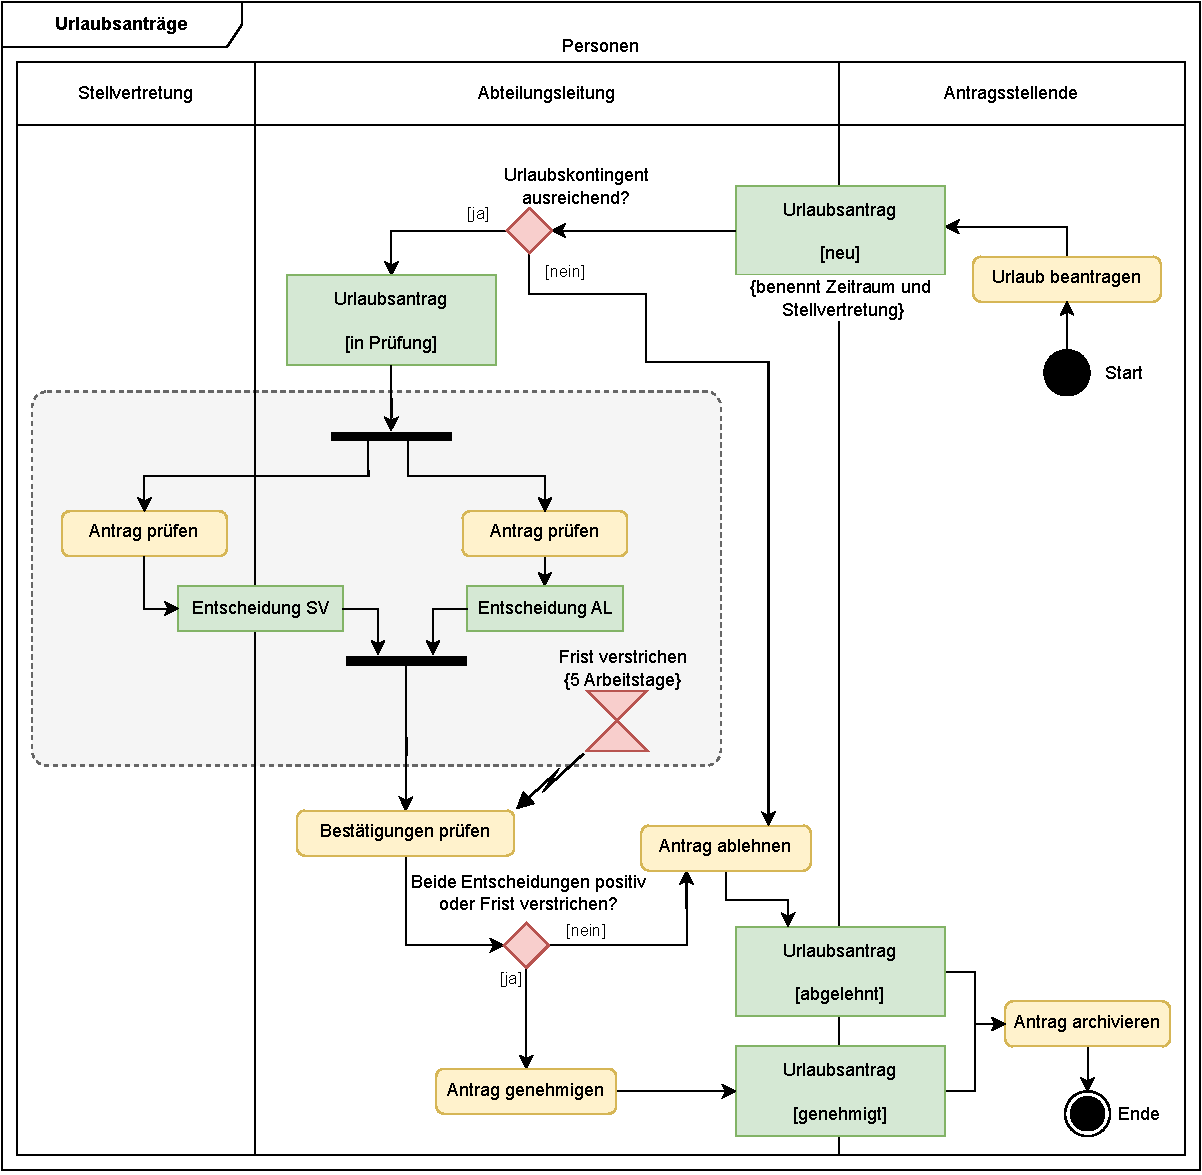
\includegraphics[width=1.0\linewidth]{h03_A2.pdf}
    }
    \caption{Lösung der Aufgabe 2}
    \label{fig:lgs2}
\end{figure}


\end{document}
